\chapter{Design}
\label{chap:structure}
The flowchart presented in the introduction of this document 
represents the macro components making up the design of \Atlas
and reflects closely the capabilities of \Atlas. We subdivide this 
chapter in various sections, each of them representing one 
of the components in \fig{fig:intro-schematics}. The order in 
which these components will be presented starts from the grid 
and closes with the numerics. Note that some simple examples 
are provided as part of this user-guide in \parte{p:core-functionalities}.


\section{Grid}
%
The Grid object forms the base class of a hierarchical inheritance tree 
as shown in \fig{fig:grids}. A Grid implementation may be structured or
unstructured. The Grid base class interface gives the capability to 
list the coordinates representing the points of a given grid, and how many
points exist in a given grid. It has no knowledge of any domain decomposition
or parallelisation in general.
The grids that \Atlas constructs can be \textit{global} or 
\textit{local}. The \textit{GlobalGrid} type represents a complete
spherical grid, whereas the \textit{LocalGrid} type represents a limited 
area of the sphere. Both global and local grids can be either 
structured or unstructured. In \fig{fig:grids} we show the 
various derived classes of the Grid class.
%
\begin{figure}[htb]
\centering
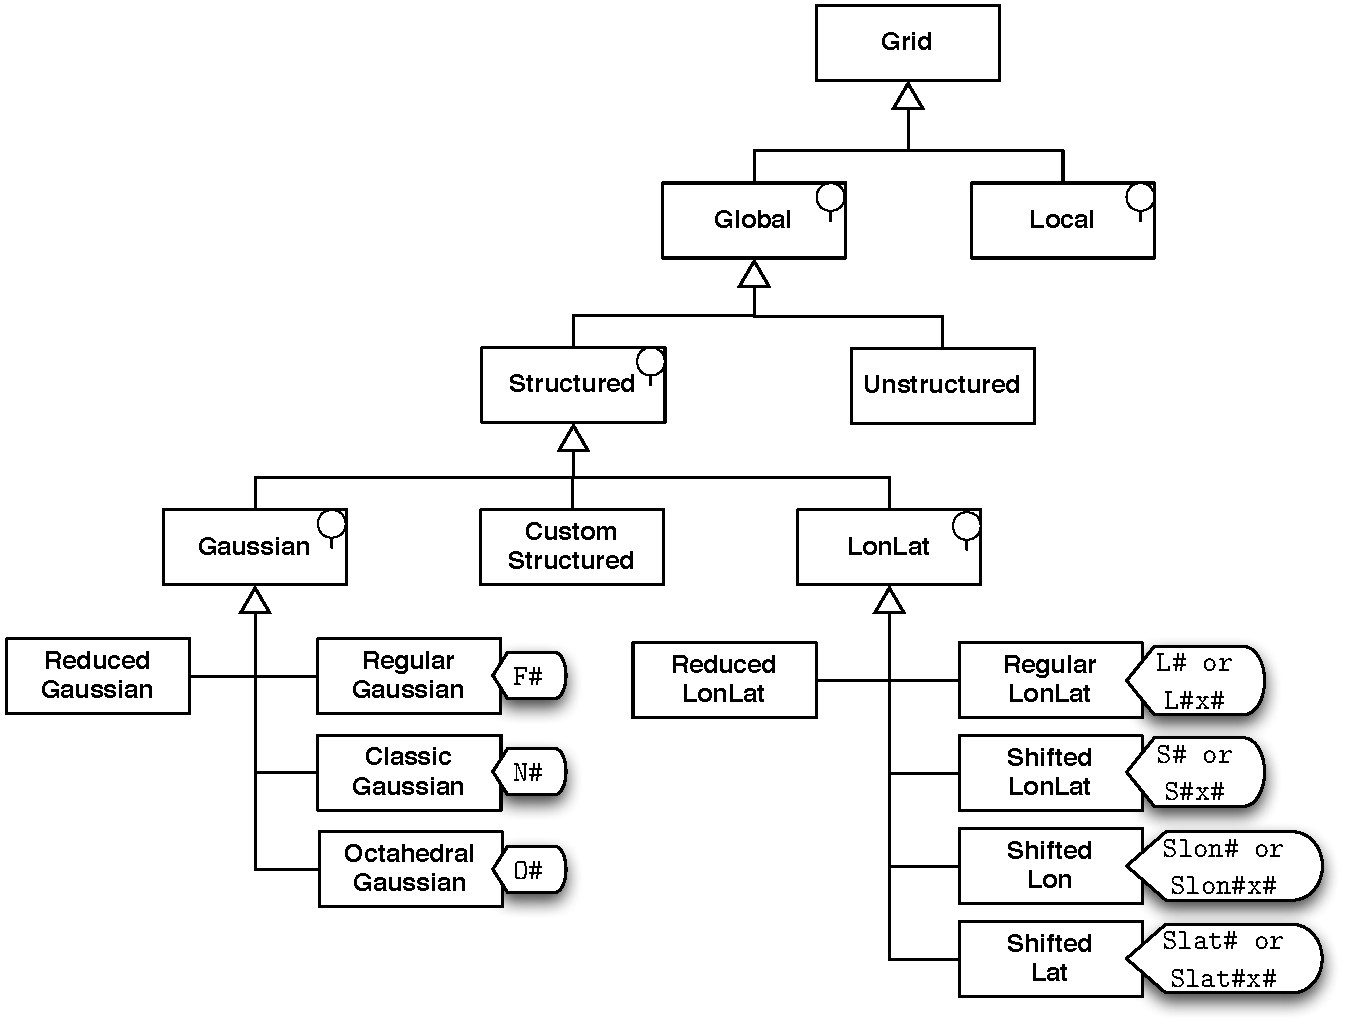
\includegraphics[width=\textwidth]{imgs/grids.pdf}
\label{fig:grids}
\caption{Grid class hierarchy.}
\end{figure}
%
Focussing on the Global grid classification, there exist several
possible sub classifications, such as the following derived types: 
\begin{itemize}
  \setlength\itemsep{0.4em}
  \item Unstructured --- No structure is present in the grid
  \item Structured --- The grid has a structured distribution of latitudes, and on each latitude a uniform distribution in zonal direction (constant $\Delta\lambda$ for one latitude). No assumption is made on the location of latitudes, or the first longitude value on one latitude.
\end{itemize}
The Structured serves as the base class for three additional derived types:
\begin{itemize}
  \setlength\itemsep{0.4em}
  \item CustomStructured --- To instantiate a customised Structured grid,
        you have to use the CustomStructured concrete class. Any of the
        following grids could be expressed as a CustomStructured grid as well.
  \item Gaussian --- The grid's latitude distribution follows the
        roots of Legendre polynomials. The resolutions of these grids are
        usually expressed by a number, describing the number of latitudes
        between a pole and the equator.
  \item LonLat --- The grid's latitude distribution is uniform.
\end{itemize}
The Gaussian grid, in turn, serves as the base class for 
\begin{itemize}
  \item RegularGaussian --- also referred to as \emph{full} Gaussian grid.
        This Gaussian grid has a constant number of points on each latitude, 
        equal to $4\ N$, with $N$ the Gaussian number or number of latitudes
        between pole and equator.
  \item ClassicGaussian --- The number of points on each latitude is computed
        by optimisations involving the orthogonality of associated Legendre
        polynomials. This is a costly computations. Hence these tables have been
        pre-computed for resolutions that have been used in the past at ECMWF.
  \item OctahedralGaussian --- The number of points on each latitude
        can be inferred from triangulating a regular octahedron, projected to
        sphere. Certain modifications are required such as modifying the
        latitude locations to the roots of the Legendre polynomials.
  \item ReducedGaussian --- The number of points on each latitude can be 
        configured by the user.
\end{itemize}
The LonLat grid class, in turn, serves as the base class for 
\begin{itemize}
  \item RegularLonLat --- This grid has a constant number of points on each
        latitude, and includes typically the pole and the equatorial latitudes,
        and the Greenwich meridian.
  \item ShiftedLonLat --- This grid has a constant number of points on each
        latitude, but is shifted half of a longitude increment and half of a
        latitude increment compared to the RegularLonLat grid. This grid can
        also be referred to as the dual grid of the RegularLonLat grid. It does
        not include pole and equatorial latitudes, and not the Greenwich 
        meridian.
  \item ShiftedLat --- This grid has a constant number of points on each
        latitude, but is shifted half of a latitude increment. It does
        not include pole and equatorial latitudes, but includes the Greenwich
        meridian.
  \item ShiftedLon --- This grid has a constant number of points on each
        latitude, but is shifted half of a longitude increment compared to the
        RegularLonLat grid. It includes pole and equatorial latitudes, but not 
        the Greenwich meridian.
  \item ReducedLonLat --- The number of points on each latitude can be 
        configured by the user. Typically these grids include the pole
        latitudes, and the Greenwich meridian.
\end{itemize}

We note that the object-oriented construction of the Grid 
object allows one to add any other grid that might be of 
interest without disrupting the existing grid workflow.


\section{Mesh} \label{s:mesh}
%
The \emph{Mesh} object describes how grid points are connected via lines,
essentially forming elements such as triangles, quadrilaterals, \ldots~
Furthermore, the \emph{Mesh} can be distributed across MPI tasks, called
partitions.
%
A \emph{Mesh} object has no inherent notion of structure. Therefore, 
the nodes and elements in a mesh partition, even if originating from
a structured grid could be in any order, and should be treated as such.
A \emph{Mesh} is composed of \emph{Nodes}, \emph{Cells}, and \emph{Edges}.
These components each contain information stored in \emph{Field}s and 
\emph{Connectivity} tables. In \fig{fig:mesh} we show the composition
of a \emph{Mesh} object. Due to the distributed nature of the mesh,
three specific fields are required in the \emph{Nodes}, \emph{Cells}
and \emph{Edges}, i.e.~the \inltc{global\_index}, \inltc{remote\_index},
and \inltc{partition}. More on parallelisation is presented in
section~\ref{s:parallelisation}.
%
\begin{figure}
\centering
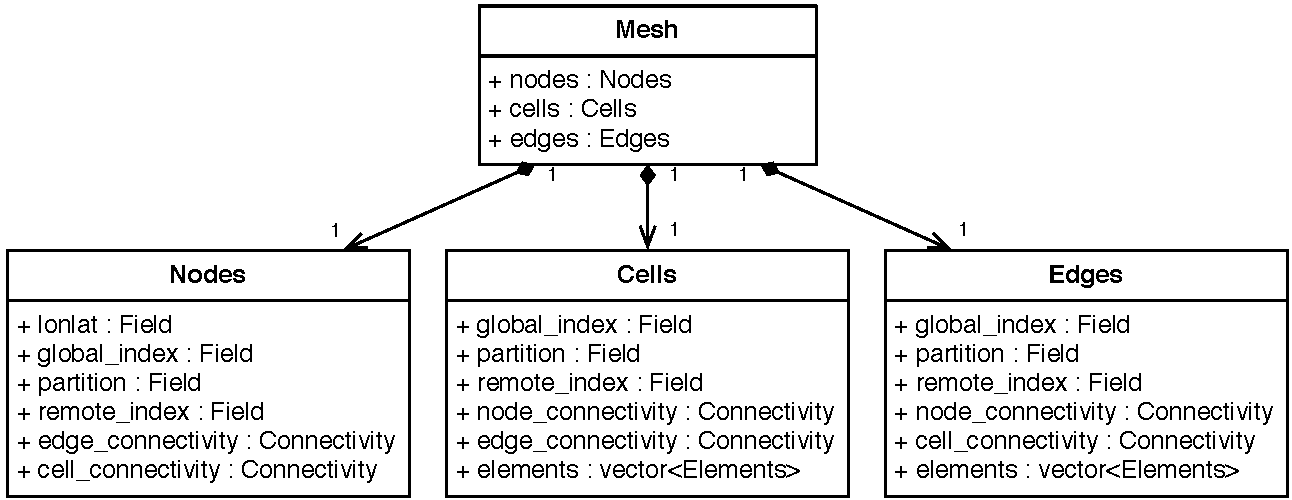
\includegraphics[width=\textwidth]{imgs/mesh.pdf}
\caption{Mesh object composition \label{fig:mesh}}
\end{figure}
%
\begin{warningbox}
Note that a mesh is not equal to a grid. The grid describes globally the list
of points without elements and connectivities, while a mesh is a list of nodes
with specific connectivity rules, forming elements, and is distributed among
MPI tasks. Note also that, in \Atlas, the number of points of a grid is
generally different from the number of nodes of a mesh.
\end{warningbox}

\subsection{Nodes}
%
The \emph{Nodes} contains a \emph{Field} called \inltc{lonlat} which contains
the coordinates of the nodes on the sphere in longitude and latitude
degrees. Apart from the \inltc{lonlat} field, any \emph{Field} which relates
to the mesh nodes can be stored in the \emph{Nodes} object. The \emph{Nodes}
therefore can also be seen as a specialised \emph{FieldSet}
(see section~\ref{s:field-fieldset}).\\
%
Also stored in the \emph{Nodes} object are connectivity tables relating the
mesh nodes to edges and/or elements present in the mesh. These tables are
only allocated upon request.

\subsection{Elements and Connectivity}
%
As depicted in \fig{fig:elements}, the \emph{Cells} and \emph{Edges} classes
derive from a class \emph{HybridElements}. The reason for the naming
\emph{hybrid} refers to the possibility of having groups of elements with
different element types present under the same umbrella. One group of elements
sharing the same \emph{ElementType} is accessible through the \emph{Elements}
class. The \emph{HybridElements} class on the other hand offers access to all
elements irrespective of their \emph{ElementType}. It could be advantageous for
an algorithm to loop over \emph{Elements} corresponding to one
\emph{ElementType}, and apply specialised instructions in a nested loop
applicable to all elements of that specific \emph{ElementType}.\\
\begin{figure}
\centering
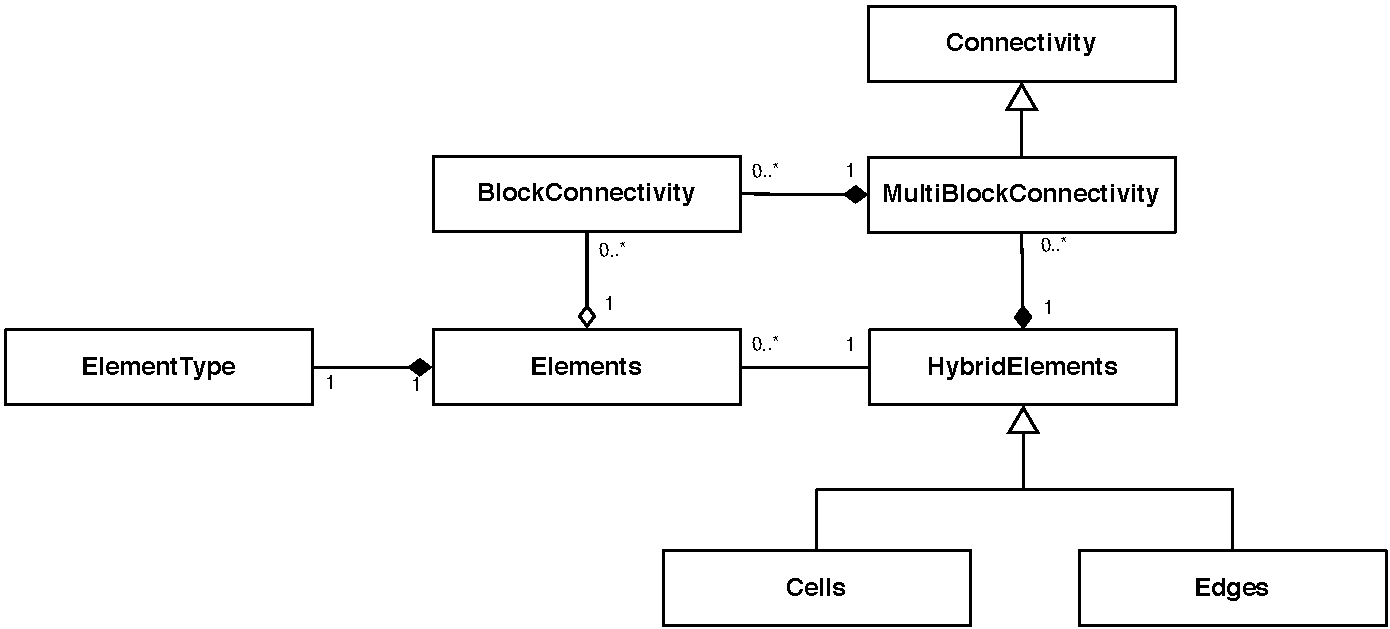
\includegraphics[width=\textwidth]{imgs/elements.pdf}
\caption{Class diagram related to the mesh \emph{Edges} and \emph{Cells}
\label{fig:elements}}
\end{figure}
Because of grouping of elements per \emph{ElementType}, \emph{Connectivity}
tables that e.g.~relate elements to nodes have the appearance of blocks. To
clarify, imagine 2 triangular elements and 3 quadrilateral elements. The table
of connectivities represented by the \emph{MultiBlockConnectivity} class would
have the form:\\[10pt]
\begin{minipage}{\textwidth}
\begin{verbatim}
                    element 1:    x  x  x
                    element 2:    x  x  x
                    element 3:    x  x  x  x
                    element 4:    x  x  x  x
                    element 5:    x  x  x  x
\end{verbatim}
\end{minipage}\\[10pt]
This \emph{MultiBlockConnectivity} table, can also be interpreted by two \emph{BlockConnectivity} tables:\\[10pt]
\begin{minipage}{\textwidth}
\begin{verbatim}
            block1, element 1:    x  x  x
            block1, element 2:    x  x  x
                                 
            block2, element 1:    x  x  x  x
            block2, element 2:    x  x  x  x
            block2, element 3:    x  x  x  x
\end{verbatim}
\end{minipage}\\[10pt]
Multiple \emph{BlockConnectivity} tables share exactly the same memory as the
one \emph{MultiBlockConnectivity} which is stored in the \emph{HybridElements}.
The \emph{Elements} objects, which are also stored in the \emph{HybridElements}
and each hold a \emph{BlockConnectivity}, therefore don't occupy any 
significant memory.

\subsection{Mesh generation}
%
The mesh is constructed using the class \emph{MeshGenerator} which can generate
a mesh taking as input a \emph{Grid}, and and optionally a
\emph{GridDistribution}. The \emph{GridDistribution} describes for each grid
point which MPI task or partition the point belongs to. If the
\emph{GridDistribution} is not given, the \emph{MeshGenerator} will internally
create a temporary \emph{GridDistribution} internally. More on this can be
found in section~\ref{s:parallelisation}.
The \emph{MeshGenerator} base class can have several concrete implementations.
Depending on the \emph{Grid} type used, some concrete implementations may not
be available. For \emph{Structured} grid types, the
\emph{mesh::generators::Structured} is available. This mesh generator is very
fast as it can take advantage of the structured nature of a \emph{Structured}
grid. For any \emph{Grid}, a slower \emph{Delaunay} triangulation is also
available.\\
%
Figure~\ref{fig:meshgen} shows the usage and class diagram of the
\emph{MeshGenerator}.
%
\begin{figure}
\centering
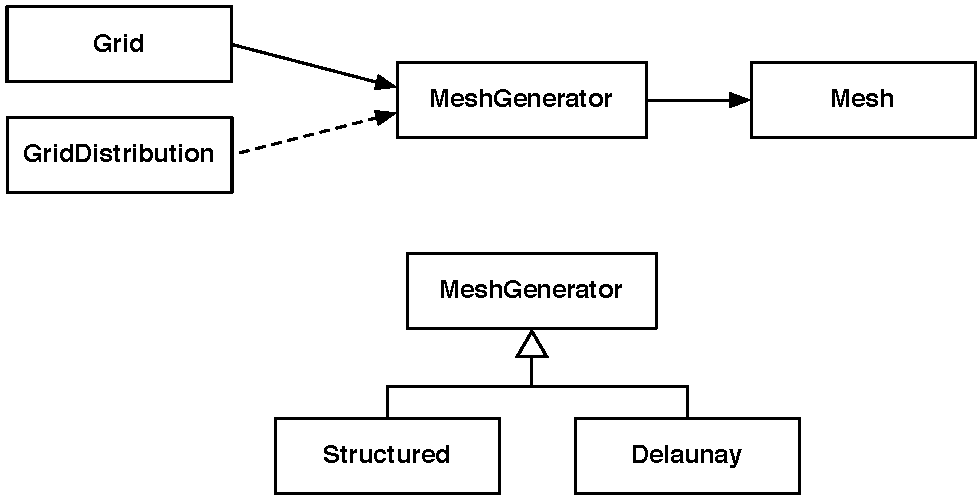
\includegraphics[scale=0.5]{imgs/meshgenerator.pdf}
\caption{Mesh generation workflow, and \emph{MeshGenerator} class diagram
\label{fig:meshgen}}
\end{figure}


\section{Field and FieldSet} \label{s:field-fieldset}
%
\emph{Field} objects encapsulate given fields, such as the temperature 
or the pressure, and they can be grouped into FieldSets.
The class diagram of the field object is depicted in \fig{fig:field}.
%
\begin{figure}
\centering
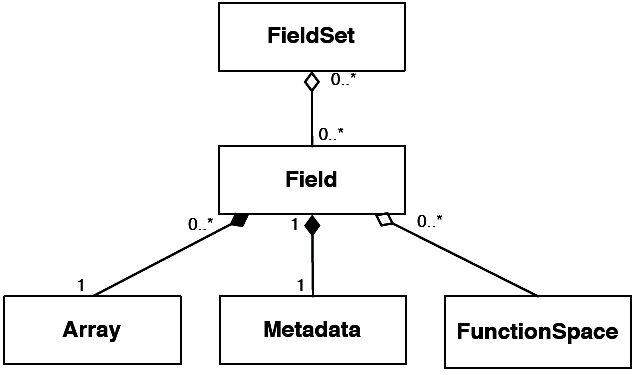
\includegraphics[scale=0.25]{imgs/field.png}
\label{fig:field}
\caption{Field and FieldSet object composition}
\end{figure}
%
In particular the \emph{Field} object is composed of 
the \emph{Array} object which contains the actual field data, and the
\emph{Metadata} object which contains descriptions of the field.
A \emph{Field} also contains a reference to a \emph{FunctionSpace} object, 
described section~\ref{s:functionspace}.

\section{FunctionSpace} \label{s:functionspace}
%
The \emph{FunctionSpace} defines how a \emph{Field} is represented on the
domain. There exist a variety of possible function spaces. Examples include 
\emph{functionspace::Spectral}, \emph{functionspace::StructuredColumns}, \emph{functionspace::NodeColumns}, and \emph{functionspace::EdgeColumns}.
These are illustrated in the \emph{FunctionSpace} class inheritance diagram in \fig{fig:functionspace}.
\begin{itemize}
  \item \emph{functionspace::Spectral} describes the discretisation in terms of         spherical harmonics. The parallelisation (gathering and scattering) in
        spectral space is delegated to a \emph{Trans} object ( in turn
        delegating to the IFS trans library)
  \item \emph{functionspace::StructuredColumns} describes the discretisation
        of distributed fields on a \emph{Structured} grid. At the moment the
        \emph{Structured} must be a \emph{Gaussian} grid for parallel
        usage as a \emph{Trans} object is responsible for the parallelisation.
        In a future release this will be generalised to use a 
        \emph{GatherScatter} object instead, which does not rely on having a 
        \emph{Gaussian} grid.\\
        \emph{Field}s described using this function space may also be defined  
        to have levels.
  \item \emph{functionspace::NodeColumns} describes the discretisation of fields
        with values colocated in the nodes of a \emph{Mesh}, and may have
        multiple levels defined in a vertical direction. These fields may have
        parallel halo's defined. A \emph{HaloExchange} object and
        \emph{GatherScatter} object are responsible for parallelisation.
  \item \emph{functionspace::EdgeColumns} describes the discretisation of fields
        with values colocated in the edge-centres of a \emph{Mesh}, and may have
        multiple levels defined in a vertical direction. These fields may have
        parallel halo's defined. A \emph{HaloExchange} object and
        \emph{GatherScatter} object are responsible for parallelisation.
\end{itemize}
%
\begin{figure}
\centering
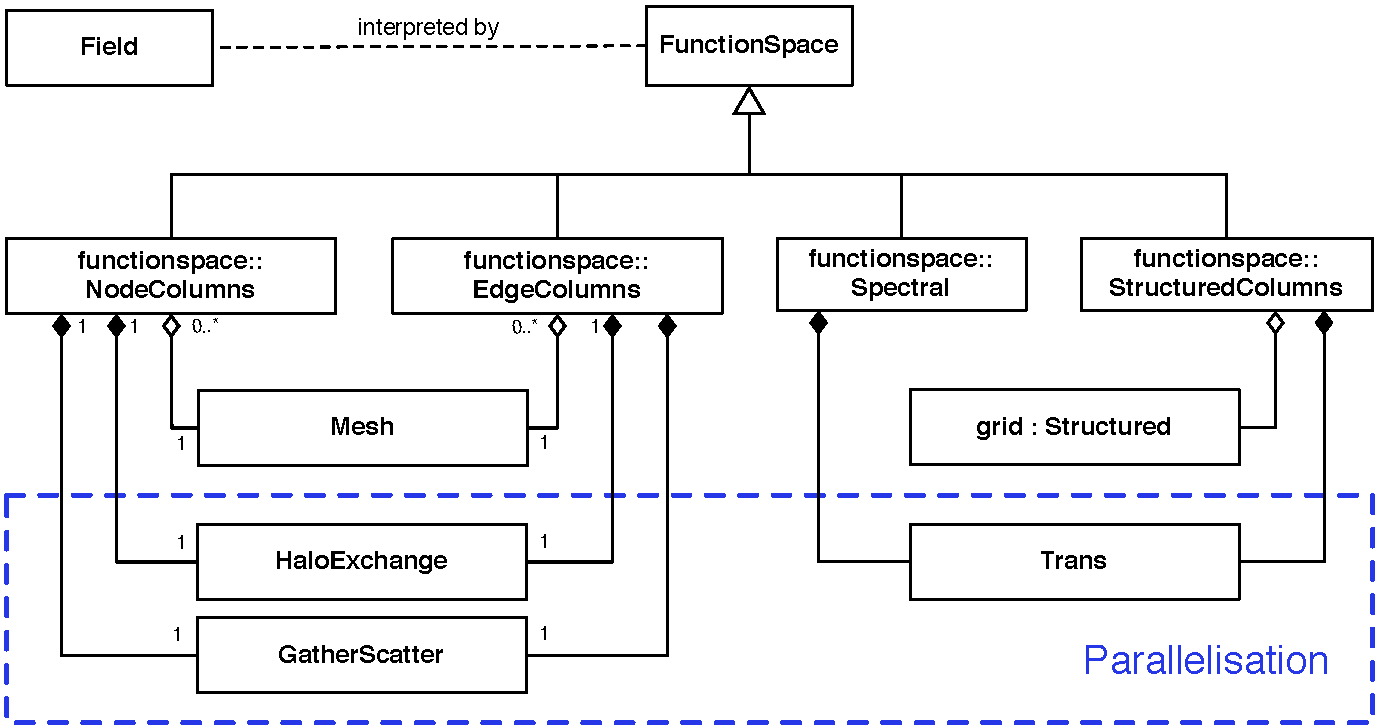
\includegraphics[width=\textwidth]{imgs/functionspace.pdf}
\caption{FunctionSpace object diagram \label{fig:functionspace}}
\end{figure}
%
\section{Parallelisation} \label{s:parallelisation}
%
As described section~\ref{s:mesh} and shown in \fig{fig:mesh}, the \emph{Nodes},
\emph{Cells}, and \emph{Edges} contain three fields related to parallelisation:
\begin{itemize}
  \item \inltc{global\_index} --- This \emph{Field} contains for each
        node or element in the mesh partition a unique global index
        or ID as if the mesh was not distributed. 
        This global index is independent of the number of partitions
        the mesh is distributed in.
  \item \inltc{partition} --- This \emph{Field} contains for each node
        or element the partition index that has ownership of the node
        or element. Nodes or elements whose partition does not match
        the partition index of the mesh partition are also called
        ghost nodes or ghost elements respectively. These ghost entities
        merely exist to facilitate stencil operations or to complete
        e.g. a mesh element.
   \item \inltc{remote\_index} --- This \emph{Field} contains for each
        node or element the local index in the mesh partition with index
        given by the \inltc{partition} field.
\end{itemize}
With the knowledge of \inltc{partition} and \inltc{remote\_index}, we now
know for each element or node which partition owns it, and at which location.
Usually the user has not to be aware of these three fields as they are
more required for \Atlas' internal parallelisation capabilities.\\
%
\Atlas has two parallel communication pattern classes that can be setup to
store how data can be sent and received between MPI tasks.
\begin{itemize}
\item The \emph{GatherScatter} class stores the communication pattern of 
gathering all data to one MPI task, and the inverse, scattering or distributing 
all data from one MPI task to all MPI tasks.
\item The \emph{HaloExchange} class stores the communication pattern of sending 
and receiving data to nearest neighbour (in domain decomposition sense) MPI 
tasks, typically required in exchanging small halo's of ghost entities 
surrounding a domain partition.
\end{itemize}
%
\section{Numerics}
%
Apart from serving as a framework for constructing a flexible data structure,
\Atlas also provides some numerical algorithms such as gradient, divergence,
curl, and laplacian operators.
%
The gradient, divergence, curl and laplacian operators are bundled in a
abstract \emph{Nabla} class, of which a concrete implementation can be
instantiated with a \emph{Method} object. This is illustrated in
\fig{fig:numerics}. Here a concrete \emph{fvm::Nabla} is constructed using a
concrete \emph{fvm::Method}. These concrete classes implement a median-dual
finite volume method. The \emph{fvm::Method} internally uses two
\emph{FunctionSpace}s, i.e. a \emph{functionspace::NodeColumns}, and a
\emph{functionspace::EdgeColumns}, required to interprete \emph{Field}s
residing in nodes and edge-centres. For more information on the median-dual
Finite Volume Method, see section~\ref{s:fvm}.
%
\begin{figure}
\centering
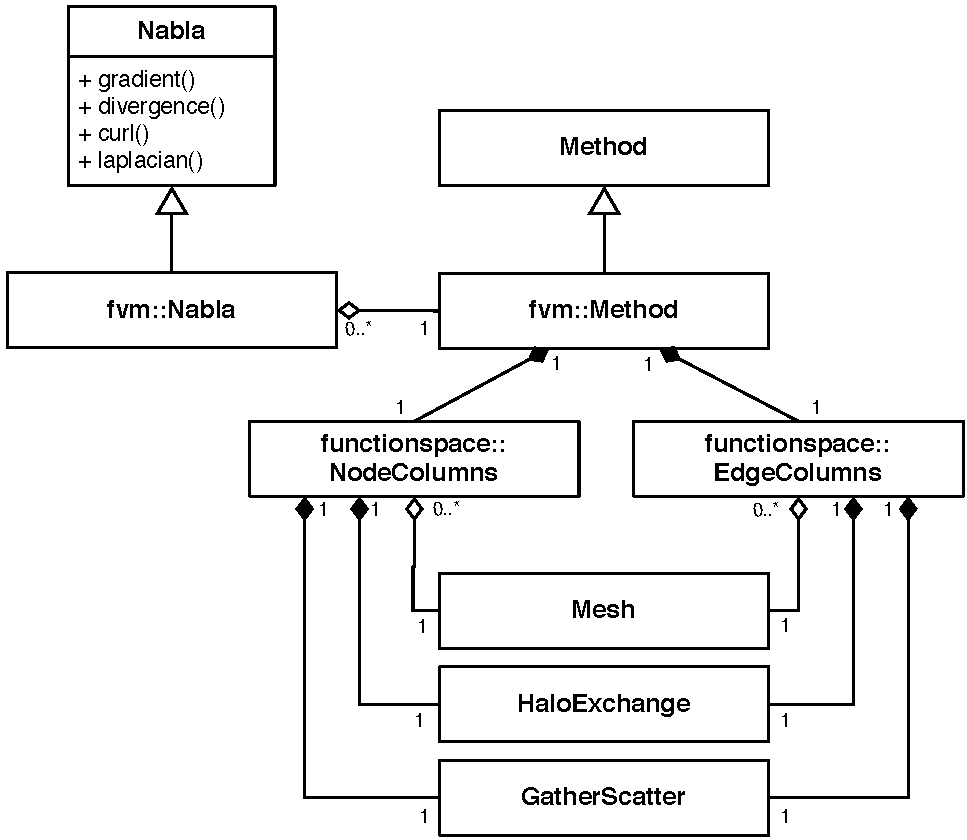
\includegraphics[scale=0.5]{imgs/numerics.pdf}
\caption{Class diagram for the \emph{fvm::Nabla} operator
\label{fig:numerics}}
\end{figure}
%
\section{Utilities}
%
A number of utilities is also available \Atlas. These include 
emph{Mesh}
writing, mpi communication, error and exception 
handling, runtime behaviour, etc.
%

\subsection{Configuration}


\subsection{Logging} \label{s:utilities-logging}
TODO

\chapter{Theory}
\section{fvm: Median-dual Finite Volume Method}
\label{s:fvm}
TODO



